%--------------------------------------------------------------------------%
%
%	This file 'Form-2.tex' is for drafting Indian patent specifications           
% 
% 	Author: Nettimi Satya Sai Srinivas
%  	E-mail: satyasaisrinivas.nettimi@gmail.com
%   
%	This work may be distributed and/or modified under the
% 	conditions of the LaTeX Project Public License, either
% 	version 1.3 of this license or (at your option) any
% 	later version.
% 	The latest version of the license is in
% 	http://www.latex-project.org/lppl.txt
% 	and version 1.3 or later is part of all distributions of
% 	LaTeX version 2003/06/01 or later.
% 
% 	This work consists of the files listed in the README file.
%
%--------------------------------------------------------------------------%

% Do not modify the code beyond this line unless specified

\documentclass[10pt, a4paper]{article}

%------------------------%
% Include LaTeX packages %
%------------------------%

  	\usepackage[top=4cm, left=4cm, bottom=3cm, right=3cm]{geometry}
%  	\usepackage{showframe}	
  	
  	\usepackage[nodisplayskipstretch]{setspace}

	\usepackage[pagewise, modulo, displaymath, mathlines]{lineno}
	\renewcommand{\linenumberfont}{\normalfont\bfseries\small}
			
	\usepackage{amsmath}
	\usepackage{amsfonts}	
	\usepackage{amssymb}
	
	\usepackage{graphicx}
	
	\usepackage{longtable}
	\usepackage{tabularx}

	\usepackage{booktabs}		
	\renewcommand{\arraystretch}{2}
	
	\usepackage{caption}	
	\captionsetup[figure]{name={FIG.},  labelsep=space, justification=raggedright, singlelinecheck=false}	
	\captionsetup[table] {name={TABLE}, labelsep=period}	

	\usepackage{enumitem}
	
	% User to set the document mode as draft or final
	\usepackage[draft, authormarkup=none, defaultcolor=red, commentmarkup=uwave]{changes}
	
%-----------------%		
% Form-2 Document %
%-----------------%

\begin{document}

	% Cover Page
	% Do not modify the code beyond this line unless specified



% Cover page begins

\begin{center}
	
	\thispagestyle{empty} 
	\textbf{FORM 2} 
	\vskip 40 pt 
	\textbf{THE PATENTS ACT, 1970}\\
	\textbf{(39 of 1970)}\\
	\textbf{\&}\\
	\textbf{The Patents Rules, 2003}
	\vskip 40 pt
	\textbf{COMPLETE SPECIFICATION}\\
	\textbf{(See section 10 and rule 13)}
	\vskip 40 pt
	\MakeUppercase{\textbf{Title of the Invention}}
	\vskip 10 pt
	\MakeUppercase
	{ 
		%----------------------%
		% User to add text here
			(Write the title of your invention) 
		% Text ends
		%----------------------%							
	}
	\vskip 40 pt
	\MakeUppercase{\textbf{Applicant}}
	\vskip 10 pt
	\textbf
	{
		%----------------------%
		% User to add text here
			(Write the name of your applicant) 
		% Text ends
		%----------------------%							
	}
	\vskip 10 pt
	{	
		%----------------------%
		% User to add text here
			(Write the communication address of your applicant)
		% Text ends
		%----------------------%							
	} 
	\vskip 10 pt

	\vspace*{\fill}
	\MakeUppercase{\textbf{Preamble to the description}}
	\vskip 10pt
	The following specification particularly describes the invention \\and the manner in which it is to be performed.
	
\end{center}

% Cover page ends
	
	\clearpage
	\newpage
	
	\linenumbers
	\doublespacing

	% Field of the Invention
	\section*{{\MakeUppercase{\normalsize Field of the Invention}}}
	% Field of the invention begins




The present invention relates to 
%----------------------%
% User to add text here
	...
% Text ends
%----------------------%




The present invention provides
%----------------------%
% User to add text here
	...
% Text ends
%----------------------%




% Field of the invention ends

	% Background of the Invention
	\section*{{\MakeUppercase{\normalsize Background of the Invention}}}
	% Background of the invention begins




%----------------------%
% User to add text here
	(Write the background of the invention)
% Text ends
%----------------------%




% Background of the invention ends

	% Objects of the Invention
	\section*{{\MakeUppercase{\normalsize Objects of the Invention}}}
	% Objects of the invention begins




The principal object of this invention is 
%----------------------%
% User to add text here
	...
% Text ends
%----------------------%




Another object of this invention is 
%----------------------%
% User to add text here
	...
% Text ends
%----------------------%




A further object of this invention is
%----------------------%
% User to add text here
	...
% Text ends
%----------------------%




%--------------------------------------------------------------------------%
% Add the preamble "A further object of this invention is" 
% at the beginning of each paragraph describing an object of the invention
%--------------------------------------------------------------------------%




% Objects of the invention ends

	% Summary of the Invention
	\section*{{\MakeUppercase{\normalsize Summary of the Invention}}}
	% Summary of the invention begins




In one aspect of the present invention,  
%----------------------%
% User to add text here
	...
% Text ends
%----------------------%




According to another aspect of the present invention, 
%----------------------%
% User to add text here
	...
% Text ends
%----------------------%




%-------------------------------------------------------------------------%
% Add the preamble "According to another aspect of the present invention" 
% at the beginning of a paragraph describing an aspect of the invention
%-------------------------------------------------------------------------%




% Do not modify beyond this line
The summary of the invention does not necessarily disclose all the inventive features. The invention may reside in a sub-combination of the disclosed features. One can understand the present invention by reference to the detailed description taken with the accompanying drawings.




% Summary of the invention ends

	% Brief Description of the Invention
	\section*{{\MakeUppercase{\normalsize Brief Description of Drawings}}} 
	% Brief description of drawings begins




A detailed description of the present invention is provided hereinbelow with reference to the following drawings in which:

FIG.~1 illustrates 
%----------------------%
% User to add text here
	...
% Text ends
%----------------------%




FIG.~2 illustrates
%----------------------%
% User to add text here
	...
% Text ends
%----------------------%




%------------------------------------------------------------------------------------%
% Add the preamble "FIG.~X illustrates" at the beginning of a new figure description %
%------------------------------------------------------------------------------------%




% Do not modify beyond this line
It is worth noting that the drawings illustrate the embodiments of the present invention with examples. The similar references in drawings denote similar components. The description and drawings are only for illustration. They serve as an aid for understanding, and they do not intend to be the definition of the limits of the invention.




% Brief description of drawings ends

	% Detailed Description of the Invention
	\section*{{\MakeUppercase{\normalsize Detailed Description of the Invention}}}
	The following description with reference to the accompanying drawings is provided to assist in a comprehensive understanding of various embodiments of the disclosure as defined by the claims and their equivalents. \\

% Detailed description of the invention begins




\noindent
METHOD




%----------------------%
% User to add text here
	\noindent
	(Disclose the best method of performing the invention which is know to the applicant and for which he is entitled to claim protection)\\
% Text ends
%----------------------%




\noindent
SYSTEM




%----------------------%
% User to add text here
	\noindent
	(Fully and particularly describe the invention and its operation or use)\\
% Text ends
%----------------------%




\noindent
INVENTIVE STEP OF THE PRESENT INVENTION\\
The inventive features of the present invention that involves technical advance as compared to the existing knowledge are briefly listed as follows:




%----------------------%
% User to add text here
	...\\
% Text ends
%----------------------%




\noindent
ADVANTAGES OF THE PRESENT INVENTION \\
The advantages of the present invention over the relevant prior art are briefly listed as follows:




%----------------------%
% User to add text here
	...\\
% Text ends
%----------------------%




\noindent
INDUSTRIAL APPLICATIONS OF THE PRESENT INVENTION \\
The present invention has numerous industrial applications, including, but not limited to,




%----------------------%
% User to add text here
	...\\
% Text ends
%----------------------%




% Detailed description of the invention ends
	
	\clearpage
	\newpage

	% Claims
	\noindent
	We claim:
	\begin{enumerate}[leftmargin=*]




	\item 
		%----------------------%
		% User to add text here
			(Write the first independent claim of your invention)
		% Text ends
		%----------------------%
	
	
	
	
	\item 
		%----------------------%
		% User to add text here
			
		% Text ends
		%----------------------%
	
	
	
		
	\item 
		%----------------------%
		% User to add text here
	
		% Text ends
		%----------------------%
	
	
	
	
			
	\item 
		%----------------------%
		% User to add text here

		% Text ends
		%----------------------%
	
	
	
	
		
	\item
		%----------------------%
		% User to add text here
	
		% Text ends
		%----------------------%
	
	
	
	
	
	\item 
		%----------------------%
		% User to add text here

		% Text ends
		%----------------------%
	
	
	
		
	\item
		%----------------------%
		% User to add text here

		% Text ends
		%----------------------%
	
	
	
	
			
	\item
		%----------------------%
		% User to add text here

		% Text ends
		%----------------------%
	
	
	
	
			
	\item
		%----------------------%
		% User to add text here

		% Text ends
		%----------------------%
	
	
	
	
	
	\item
		%----------------------%
		% User to add text here

		% Text ends
		%----------------------%
		
		
		
		
		%--------------------------------------------------------------------------%
		% Add \item to include a new claim
		%--------------------------------------------------------------------------%



		
\end{enumerate}

\vspace{1cm}

	%----------------------%
	% User to add text here 
	
		% Enter the details of date, month, and year
		\noindent
		Dated this x\textsuperscript{y} day of Month Year.
	
	%	Text ends
	%----------------------%




\begin{flushright}
	
	%----------------------%
	% User to add text here		
	
		% Source the signature file of the authorized signatory
		
\includegraphics[scale=0.20]{figures/signature.eps} \\	
	
	%	Text ends
	%----------------------%
	
	
	
	
	%----------------------%
	% User to add text here 
		
		% Enter the name of the authorized signatory
		% Case-1: Authorized signatory is the inventor(s), when the inventor(s) and applicant(s) are same; and no patent agent is involved.
		% Case-2: Authorized signatory is the authorized person of the applicant(s), when the inventor(s) and applicant(s) are different; and no patent agent is involved.
		% Case-3: Authorized signatory is the patent agent, by default.
	
		Name of the Authorized Signatory \\
		
	% Text ends
	%----------------------%
	
	

	
	%----------------------%
	% User to add text here 
	
		% Enter the relevant details of the authorized signatory
		% Case-1: Inventor
		% Case-2: Authorized Person for the Applicant
		% Case-3: Patent Agent for the Applicant [Patent Agent Number]
			
		Relevant Details of the Authorized Signatory \\
		
	% Text ends
	%----------------------%
	
	
	
	
\end{flushright}

	\clearpage
	\newpage

	% Abstract
	\begin{center}
		\section*{{\MakeUppercase{\normalsize Abstract}}}
	\end{center}

	% Do not modify the code beyond this line unless specified

\begin{center}
	\MakeUppercase
	{
		%----------------------%
		% User to add text here
			(Write the title of your invention)
		% Text ends
		%----------------------%	
	}
\end{center}



%----------------------%
% User to add text here
	(Write the abstract of the invention)
% Text ends
%----------------------%
	
	
	
	
%----------------------%
% User to add text here

	% Set the figure counter value to (n-1), 
	% where n refers to FIG. n, i.e., main figure of the invention, present in the drawing sheets 
	% that accompanies the provisional/complete specifications
	
	\setcounter{figure}{22}
% Text ends
%----------------------%




\vfill
\begin{figure}[h!]
	\centering
	
	
	
	
	%----------------------%
	% User to add text here	
		
		% Source the abstract FIG file
		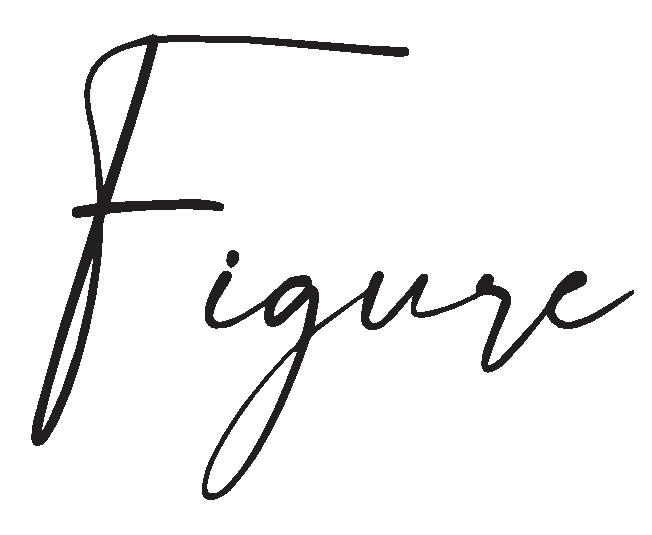
\includegraphics[scale=0.50]{figures/figure.eps}
	% Text ends
	%----------------------%
	
	
	
	
	\caption{}
\end{figure}
	
\end{document}
